\chapter{Agenti logici:\ la logica del prim'ordine}

Nella logica dei predicati abbiamo assunzioni ontologiche più ricche:\ gli \textit{oggetti}, le \textit{proprietà} e le \textit{relazioni}.\
Si inizia con una \textbf{\textit{concettualizzazione}}:\ si tratta di decidere quali sono le cose di cui si vuole parlare.
\begin{itemize}
	\item Gli \textit{oggetti}:\ un libro, un evento, una persona, un istante di tempo, un insieme, una funzione, un unicorno\dots
	      Gli oggetti possono essere identificati con simboli o relativamente ad altri oggetti, mediante \textit{funzioni} (``\textit{la madre di Pietro}''); l'insieme degli oggetti rilevanti costituiscono il \textbf{\textit{dominio del discorso}}.\
	\item Le proprietà:\ ``\textit{la madre di Pietro è simpatica}''.
	\item Le relazioni tra gli oggetti:\ ``\textit{Pietro è amico di Paolo}''.
\end{itemize}

\subsubsection{Esempio:\ il mondo dei blocchi}

Ci interessanno i blocchi e alcune loro relazioni spaziali.\

\begin{figure}[H]
	\centering
	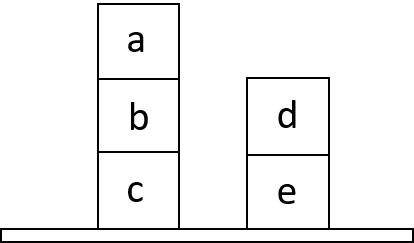
\includegraphics[width=0.4\textwidth]{immagini/mondo_blocchi.png}
\end{figure}

\noindent\textbf{\textit{Dominio}}:\ \{a, b, c, d, e\} $\leftarrow$ blocchi veri!\

\noindent Le \textbf{\textit{funzioni}}:\ si individuano le funzioni rilevanti che servono anch'esse per identificare oggetti.\ Per esempio \textit{Hat} è la funzione unaria che dato un blocco identifica il blocco che ci sta sopra:\ $Hat(b)=a$.\

\noindent Le \textbf{\textit{relazioni}}:\ si individuano le relazioni interessanti.\ Per esempio:
\begin{itemize}
	\item $On = \{\langle a, b\rangle, \langle b, c\rangle, \langle d, e \rangle\}$
	\item $Clear= \{a, d\}$
	\item $Table= \{c, e\}$
	\item $Block= \{a, b, c, d, e\}$
\end{itemize}

\[
	\langle \{a, b, c, d, e\}, \{Hat\}, \{On, Clear, Table, Block\} \rangle
\]
Le concettualizzazioni possibili sono infinite:\ un aspetto importante è il livello di astrazione \textit{giusto} per gli scopi della rappresentazione.

\section{Linguaggio}

\subsubsection{Vocabolario}
\begin{itemize}
	\item \textit{Connettivo} $\rightarrow$ $\land\ |\ \lor\ |\ \lnot\ |\ \Rightarrow\ |\ \Leftarrow\ |\ \Leftrightarrow $
	\item \textit{Quantificatore} $\rightarrow$ $\forall\ |\ \exists$
	\item \textit{Variabile} $\rightarrow$ $x\ |\ y\ |\ \dots\ |$ (lettere minuscole)
	\item \textit{Costante} $\rightarrow$ $ A\ |\ B\ |\ \dots\ |$ (lettere maiuscole)
	\item \textit{Funzione} $\rightarrow$ $Hat\ |\ Padre\textrm{-}di\ |\ +\ |\ -\ |\ \dots$ \qquad (con arità $\geq$ 1)
	\item \textit{Predicato} $\rightarrow$ $On\ |\ Clear\ |\ \geq\ |\ \leq\ |\ \dots$ \qquad (con arità $\geq$ 0)
\end{itemize}

\noindent \textbf{Nota}:\ l'ordine dei quantificatori è importante

\begin{table}[H]
	\centering
	\begin{tabular}{l l}
		$\forall x\ (\exists y\ Ama(x,y))$ & \textit{Tutti amano qualcuno}           \\
		$\exists x\ (\forall y\ Ama(x,y))$ & \textit{Esiste qualcuno amato da tutti} \\
	\end{tabular}
\end{table}

\subsubsection{I termini}

La sintassi dei termini:\
\begin{table}[H]
	\centering
	\begin{tabular}{l l}
		\textit{Termine} $\rightarrow$ & $Costante\ |\ Variabile\ |\ Funzione (Termine,\ \dots)$ \\
		                               & (un numero di termini pari alla arità della funzione)   \\
	\end{tabular}
\end{table}

\subsubsection{Le formule}

La sintassi delle formule:

\begin{table}[H]
	\centering
	\begin{tabular}{l l p{18em}}
		Formula-atomica & $\rightarrow$ & $ True\ |\ False\ |$                                                         \\
		                &               & $Termine = Termine\ |$                                                       \\
		                &               & $Predicato (Termine,\ \dots)$                                                \\
		                &               & (un numero di termini pari alla arità del predicato)                         \\
		Formula         & $\rightarrow$ & $Formula\textrm{-}atomica\ | \newline Formula\ Connettivo\ Formula\ |$       \\
		                &               & $Quantificatore\ Variabile\ Formula\ | \newline \lnot Formula\ |\ (Formula)$ \\
	\end{tabular}
\end{table}

\noindent Di solito le variabili sono usate nell'ambito di quantificatori.\ In tal caso le occorrenze si dicono \textbf{\textit{legate}}.\ Se non sono legate allora sono \textbf{\textit{libere}}.

\begin{table}[H]
	\centering
	\begin{tabular}{l l}
		$ Mela(x) \Rightarrow Rossa(x)$            & x è libera in entrambe le occorrenze \\
		$\forall x\ Mela(x) \Rightarrow Rossa(x) $ & x è legata                           \\
		$ Mela(x) \Rightarrow \exists x\ Rossa(x)$ & la prima è libera, la seconda legata \\
	\end{tabular}
\end{table}

\begin{definition}
	Una formula si dice \textbf{\textit{chiusa}} se non contiene occorrenze di variabili libere.\
	Altrimenti è detta \textbf{\textit{aperta}}.
\end{definition}

\begin{definition}
	Una formula si dice \textbf{\textit{ground}} se non contiene variabili.

\end{definition}

\subsubsection{Precedenza tra gli operatori logici}

\[
	=\ >\ \lnot\ >\ \land\ >\ \lor\ >\ \Rightarrow,\ \Leftrightarrow\ >\ \forall,\ \exists
\]

\subsection{Semantica dichiarativa}

\begin{figure}[H]
	\centering
	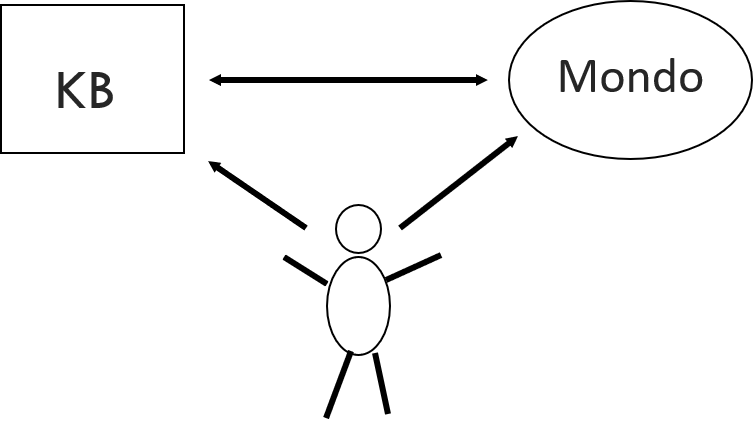
\includegraphics[width=0.4\textwidth]{immagini/Semantica_dichiarativa.png}
\end{figure}

Consiste nello stabilire una corrispondenza tra:
\begin{itemize}
	\item i termini del linguaggio e gli oggetti del mondo,
	\item le formule chiuse e i valori di verità.
\end{itemize}

\subsubsection{Interpretazione}

Una interpretazione \textbf{\textit{I}} stabilisce una corrispondenza precisa tra elementi atomici del linguaggio ed elementi della concettualizzazione.\
\textbf{\textit{I}} interpreta:
\begin{itemize}
	\item i simboli di costante come elementi del dominio;
	\item i simboli di funzione come funzioni da \textit{n-uple} di D in D;
	\item i simboli di predicato come insiemi di \textit{n-uple}.
\end{itemize}

\subsection{Semantica composizionale}

Il significato di un termine o di una formula composta è determinato in funzione del significato dei suoi componenti:
\begin{itemize}
	\item La formula A $\land$ B è vera in una certa interpretazione se entrambe A e B sono vere
	\item $\lnot$A è vera se A è falsa
	\item A $\lor$ B è vera se A è vera oppure B è vera (o entrambe)
	\item A $\Rightarrow$ B è vera se A è falsa oppure B è vera (come $\lnot$A $\Rightarrow$ B)
\end{itemize}

\subsubsection{Semantica ($\forall$)}

$\forall x\ A(x)$ è vera se per ciascun elemento del dominio A è vera.\
Se il dominio è finito equivale a un grosso $\land$.

Tipicamente $\forall$ si usa quasi sempre insieme a $\Rightarrow$:\ difficilmente una proprietà è universale, le condizioni nell'antecedente restringono la portata dell'asserzione e la qualificano.

\subsubsection{Semantica ($\exists$)}

$\exists x\ A(x)$ è vera se esiste almeno un elemento del dominio per cui A è vera.\
Se il dominio è finito equivale a un grosso $\lor$.

Tipicamente $\exists$ si usa con $\land$.

\subsubsection{Relazione tra $\forall$ e $\exists$}

Da qui discendono delle proprietà che mettono in relazione $\forall$ e $\exists$.

\begin{table}[H]
	\centering
	\begin{tabular}{l l}
		$ \forall x\ \lnot P(x) \equiv \lnot\exists x\ P(x) $ & $ \lnot P\ \land\ \lnot Q \equiv \lnot (P\ \lor\ Q) $ \\
		$ \lnot\forall x\ P(x) \equiv \exists x\ \lnot P(x) $ & $ \lnot (P\ \land\ Q) \equiv \lnot P\ \lor\ \lnot Q $ \\
		$ \forall x\ P(x) \equiv \lnot\exists x\ \lnot P(x) $ & $ P\ \land\ Q \equiv \lnot (\lnot P\ \lor\ \lnot Q)$  \\
		$ \lnot\forall x\ \lnot P(x) \equiv \exists x\ P(x) $ & $ P\ \lor\ Q \equiv \lnot (\lnot P\ \land\ \lnot Q) $ \\
	\end{tabular}
\end{table}

\subsection{Semantica ``standard'' e semantica ``database''}

Riccardo ha solo due fratelli:\ Giovanni e Goffredo.\ In logica classica:

\begin{center}
	Fratello(Riccardo, Giovanni) $\land$ Fratello(Riccardo, Goffredo)

	$\land$ Giovanni $\neq$ Goffredo $\land$

	$\forall$x Fratello(Riccardo, x) $\Rightarrow$ (x = Giovanni) $\lor$ (x = Goffredo).
\end{center}

\noindent Semantica dei database (e di alcuni linguaggi per la RC)
\begin{itemize}
	\item Ipotesi dei nomi unici:\ simboli distinti, oggetti distinti.
	\item Ipotesi del mondo chiuso:\ tutto ciò di cui non si sa che è vero è falso.
	\item Chiusura del dominio:\ esistono solo gli oggetti di cui si parla.
\end{itemize}

\subsubsection{Interazione con la KB in FOL}

Asserzioni
\begin{flushleft}
	TELL(KB, \textit{King}(\textit{John})), TELL(KB, \textit{King}(\textit{George})),

	TELL(KB, $\forall x King(x) \Rightarrow Person(x)$)
\end{flushleft}

\noindent Conseguenze logiche

\begin{flushleft}
	ASK(KB, \textit{Person}(\textit{John})) \qquad Sì, se KB $\models Person(John)$

	ASK(KB, $\exists x\ Person(x)$) \qquad ``Sì'' sarebbe riduttivo:\ la risposta è una lista di sostituzioni o legami.
\end{flushleft}

\section{Inferenza nella logica del primo ordine}

Istanziazione dell’Universale ($\forall$-eliminazione)

\[
	\frac{\forall x\ A[x]}{A[g]}
\]

\noindent dove \textit{g} è un termine \textit{ground} e A[g] è il risultato della sostituzione di \textit{g} per \textit{x} in A.

\noindent Istanziazione dell'esistenziale ($\exists$-eliminazione)

\[ \frac{\exists x\ A[x]}{A[k]} \]

\noindent Se $\exists$ non compare nell'ambito $\forall$, \textit{k}
è una costante nuova (\textit{costante di Skolem}), altrimenti va introdotta una funzione (di Skolem) nelle variabili quantificate universalmente.

\subsubsection{Riduzione a inferenza proposizionale}

Proposizionalizzazione (\textit{Grounding})
\begin{itemize}
	\item Creare tante istanze delle formule quantificate universalmente quanti sono gli oggetti menzionati.
	\item Eliminare i quantificatori esistenziali skolemizzando.
\end{itemize}

\noindent A questo punto possiamo trattare la KB come proposizionale e applicare gli algoritmi visti.\ Problemi?\ Le costanti sono in numero finito\dots ma se ci sono funzioni, il numero di istanze da creare è infinito.

\subsubsection{Teorema di Herbrand}

Se KB $\models$ A allora c'è una dimostrazione che coinvolge solo un sotto-insieme finito della KB proposizionalizzata.\
Si può procedere incrementalmente:
\begin{enumerate}
	\item creare le istanze con le costanti,
	\item creare le istanze con un solo livello di annidamento,
	\item creare quelle con due livelli di annidamento,
	\item \dots
\end{enumerate}

\noindent Se KB $\not\models$ A il processo non termina.\
Il problema è \textit{semidecidibile}.

\subsubsection{Forma a clausole}

Costanti, funzioni, predicati sono come definiti, ma escludiamo nel seguito formule atomiche del tipo ($t_1 = t_2$).\
Una clausola è un insieme di \textbf{letterali} che rappresenta la loro disgiunzione.\
Una KB è un insieme di clausole.

\subsubsection{Trasformazione in forma a clausole}

\begin{theorem}
	Per ogni formula chiusa del FOL è possibile trovare in maniera \textbf{effettiva} un insieme di clausole \textit{FC}() che è \textit{soddisfacibile} sse $\alpha$ lo era [\textit{insoddisfacibile} sse $\alpha$ lo era].\
\end{theorem}

\noindent Trasformazione:\

\begin{enumerate}
	\item Eliminazione delle implicazioni ($\Rightarrow$ e $\Leftrightarrow$).
	\item Negazioni all'interno.
	\item Standardizzazione delle variabili:\ facciamo in modo che ogni quantificatore usi una variabile diversa.
	\item Skolemizzazione:\ eliminazione dei quantificatori esistenziali.
	\item Eliminazione quantificatori universali.
	\item Forma normale congiuntiva (congiunzione di disgiunzioni di letterali).
	\item Notazione a clausole.
	\item Separazione delle variabili:\ clausole diverse, variabili diverse.
\end{enumerate}

\subsection{Unificazione e Sostituzione}

\textbf{\textit{Unificazione}}:\ operazione mediante la quale si determina se due espressioni possono essere rese \textbf{identiche} mediante una \textbf{sostituzione} di termini a variabili.\
Il risultato è la \textbf{sostituzione} che rende le due espressioni identiche, detta \textbf{\textit{unificatore}}, o FAIL, se le espressioni non sono unificabili.

\noindent\textbf{\textit{Sostituzione}}:\ un insieme finito di associazioni tra variabili e termini, in cui ogni variabile compare una sola volta sulla sinista.\

\textbf{Nota}:\ sulla sinistra solla variabili, sulla destra costanti variabili, funzioni\dots con la restrizione che una variabile sulla sinistra non può comparire anche sulla destra.

\begin{table}[H]
	\centering
	\begin{tabular}{l l}
		\{x/f(x)\}      & NO, sostituzione circolare. \\
		\{x/g(y), y/z\} & NO, non normalizzata.       \\
	\end{tabular}
\end{table}

\subsubsection{Applicazione di sostituzione}

Sia $\sigma$ una sostituzione, A un'espressione:\ A$\sigma$ istanza generata dalla sostituzione (delle variabili con le corrispondenti espressioni), in AIMA \texttt{SUBST}($\sigma$, A).\
\textbf{Nota}:\ le variabili vengono sostituite \textbf{simultaneamente} e si esegue solo un passo di sostituzione.

\subsubsection{Espressioni unificabili}

\textbf{\textit{Espressioni unificabili}}:\ se esiste una sostituzione che le rende \textbf{identiche} (\textit{unificatore}) oppure FAIL.\
Per esempio P(A,y,z) e P(x,B,z) sono unificabili con $\tau$ = \{x/A,y/B,z/C\}; $\tau$ è un unificatore, ma non l'unico\dots un altro è $\sigma$=\{x/A,y/B\}.\
$\sigma$ è \textit{più generale} di $\tau$ (istanzia ``meno'').\
Vorremmo l'\textit{unificatore più generale} di tutti (MGU) e normalizzato.\

\begin{theorem}
	L'unificatore più generale è unico, a parte i nomi delle variabili (l'ordine non conta).
\end{theorem}

\subsubsection{Algoritmo di unificazione}

L'algoritmo di unificazione prende in input due espressioni \textit{p}, \textit{q} e restituisce un MGU $\Theta$ se esiste

\begin{itemize}
	\item \texttt{UNIFY}(p,q) = $\Theta$\quad tale che \quad\texttt{SUBST}($\Theta$,p) = \texttt{SUBST}($\Theta$,q)
	\item altrimenti FAIL
\end{itemize}

\noindent L'algoritmo esplora in parallelo le due espressioni e costruisce l'unificatore strada facendo; appena trova espressioni non unificabili fallisce.\
Una causa di fallimento sono le sostituzioni del tipo x=f(x); questo controllo si chiama \textbf{\textit{occurr check}}.

\begin{figure}[H]
	\centering
	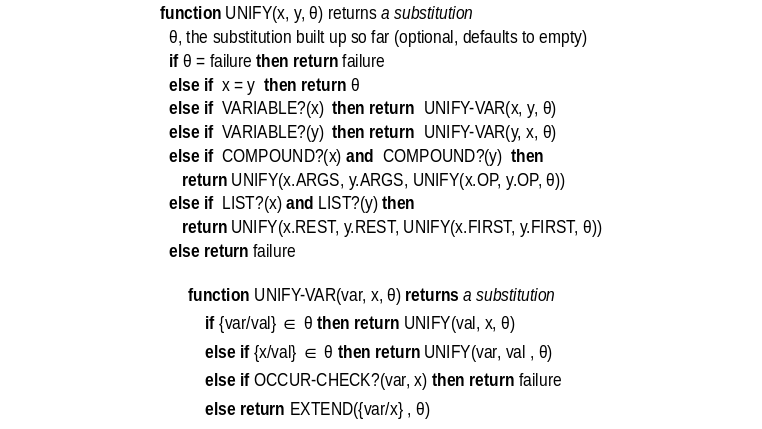
\includegraphics[width=0.8\textwidth]{immagini/sostituzione_alg.png}
\end{figure}

\noindent OCCURR-CHECK controlla se \texttt{var} occorre all'interno dell'espressione \texttt{x}, in tal caso fallisce.\
È un controllo di complessità quadratica.\
\textbf{Attenzione}:\ \texttt{EXTEND} non aggiunge semplicemente ma applica la sostituzione in $\Theta$.

\subsubsection{Problema dei fattori}
Se un sotto insieme dei letterali di una clausola può essere unificato allora la clausola ottenuta dopo tale unificazione si dice \textbf{\textit{fattore}} della clausola originaria.\
Il metodo di risoluzione va applicato ai \textit{fattori} delle clausole.\
La deduzione per risoluzione \textbf{è corretta}

\begin{center}
	\textit{Correttezza}: Se $\Gamma \vdash$\textsubscript{RES} A allora $\Gamma \models$ A
\end{center}

\noindent La deduzione per risoluzione \textbf{\textit{non è completa}}:
\begin{center}
	può essere $\Gamma \models$ A e non $\Gamma \vdash$\textsubscript{RES} A
\end{center}

\subsubsection{Risoluzione per refutazione}

Il \textit{teorema di refutazione} ci suggerisce un metodo alternativo \textbf{\textit{completo}}.

\begin{theorem}[Refutazione]
	$\Gamma \cup \{\lnot A\}$ è insoddisfacibile sse $\Gamma \models$ A.
\end{theorem}

\begin{theorem}
	$\Gamma$ è insoddisfacibile sse $\Gamma \vdash_{RES} \{ \}$.
\end{theorem}

\noindent Abbiamo un metodo \textbf{\textit{meccanizzabile}}, \textbf{\textit{corretto}} e \textbf{\textit{completo}}:\ basta aggiungere il negato della formula da dimostrare e provare a generare la clausola vuota.
